\documentclass{amsart}

\usepackage[brazilian]{babel}
\usepackage[utf8]{inputenc}
\usepackage{graphicx}
\usepackage{mathtools}
\usepackage{amsthm}
\usepackage{thmtools,thm-restate}
\usepackage{amsfonts}
\usepackage{hyperref}
\usepackage[singlelinecheck=false]{caption}
\usepackage[backend=biber,url=true,doi=true,eprint=false,style=alphabetic]{biblatex}
\usepackage{enumitem}
\usepackage[justification=centering]{caption}
\usepackage{indentfirst}
\usepackage{algorithm}
\usepackage{algpseudocode}
\usepackage{listings}

\addbibresource{references.bib}

\makeatletter
\def\subsection{\@startsection{subsection}{3}%
  \z@{.5\linespacing\@plus.7\linespacing}{.1\linespacing}%
  {\normalfont\itshape}}
\makeatother

\DeclareMathOperator*{\argmin}{arg\,min}
\DeclareMathOperator*{\argmax}{arg\,max}

\newcommand\defeq{\mathrel{\overset{\makebox[0pt]{\mbox{\normalfont\tiny\sffamily def}}}{=}}}

\algrenewcommand\algorithmicrequire{\textbf{Input}}
\algrenewcommand\algorithmicensure{\textbf{Output}}

\captionsetup[table]{labelsep=space}

\theoremstyle{plain}

\newcounter{dummy-def}\numberwithin{dummy-def}{subsection}
\newtheorem{definition}[dummy-def]{Definição}
\newcounter{dummy-thm}\numberwithin{dummy-thm}{subsection}
\newtheorem{theorem}[dummy-thm]{Teorema}
\newcounter{dummy-prop}\numberwithin{dummy-prop}{subsection}
\newtheorem{proposition}[dummy-prop]{Proposição}
\newcounter{dummy-ex}\numberwithin{dummy-ex}{subsection}
\newtheorem{exercise}[dummy-ex]{Exercício}
\newcounter{dummy-eg}\numberwithin{dummy-eg}{subsection}
\newtheorem{example}[dummy-eg]{Exemplo}

\numberwithin{equation}{subsection}

\newcommand{\set}[1]{\mathbf{#1}}
\newcommand{\pr}{\mathbb{P}}
\renewcommand{\implies}{\Rightarrow}

\newcommand{\bigo}{\mathcal{O}}

\setlength{\parskip}{1em}

\lstset{frameround=fttt,
  language=[5.3]Lua,
	numbers=left,
	breaklines=true,
	keywordstyle=\bfseries,
	basicstyle=\ttfamily,
}

\newcommand{\code}[1]{\lstinline[mathescape=true]{#1}}
\newcommand{\mcode}[1]{\lstinline[mathescape]!#1!}


\title{%
  \noindent\rule{10cm}{0.8pt}\\
  Estudo sobre Sum-Product Networks e Aprendizagem Profunda\\[1ex]
  \scriptsize\mdseries
  PTC2669 - Introdução a Inteligência Computacional\\
  Instituto de Matemática e Estatística - USP\\%
  \tiny~\\
  Relatório 1\\%
  \noindent\rule{10cm}{0.8pt}
}
\xdef\shorttitle{Sum-Product Networks e Deep Learning (Relatório 1) - Renato Geh}
%\title[]{Estudo sobre Sum-Product Networks e Aprendizagem Profunda}
\author[]{Renato Lui Geh\\NUSP\@: 8536030}

\begin{document}

\begin{abstract}
  Na área de Indecisão Probabilística, buscamos representar conhecimento por meio de distribuições
  de probabilidade. Modelos probabilísticos baseados em grafos são usados para realizar modelagem
  e raciocínio de forma compacta e tratável, já que distribuições de probabilidade têm tamanho
  exponencial no número de variáveis. No entanto, efetuar inferência exata na maioria destes
  modelos é uma tarefa NP-difícil~\cite{inference-nphard}, e portanto dependemos de técnicas de
  inferência aproximada, o que resulta em aprendizado aproximado, já que aprendizado utiliza
  inferência como subrotina. Apesar de existirem modelos onde inferência exata e tratável é
  possível, as distribuições que estes modelos conseguem representar é limitada.

  Sum-Product Networks (SPNs) são modelos em que inferência é exata e tratável. Além disso, SPNs
  são mais gerais que outros modelos exatos no sentido que SPNs conseguem representar mais
  distribuições. SPNs diferenciam-se de outros modelos probabilísticos por não terem uma sintaxe
  explícita quanto as probabilidades como Redes Bayesianas ou Redes de Markov. Sua estrutura
  assemelha-se a de uma rede neural, e portanto a derivação do algoritmo de
  \textit{backpropagation} é natural e direto. Além disso, sua arquitetura é natural a
  implementação de camadas ocultas, e portanto a \textit{deep learning}.

  Neste relatório, vamos enumerar os problemas encontrados com os chamados modelos probabilísticos
  baseados em grafo clássicos como motivação a elaboração de SPNs. Em seguida vamos mostrar de
  forma superficial a estrutura de uma SPN e fazer comparações com redes neurais artificiais.
  \vspace*{-3.5em}
\end{abstract}

\maketitle

\section{Introdução}

Considere uma distribuição de probabilidade conjunta $\Pr(\set{X}=\{X_1,\ldots,X_n\})$. Se
enumerarmos cada probabilidade de cada instanciação de $\set{X}$, teremos uma tabela da forma

\begin{table}[h]
  \begin{center}
    \begin{tabular}{c | c c c | r}
      $\set{x}^{(i)}$ & $X_1$ & $\cdots$ & $X_n$ & $\Pr(x_1,\ldots,x_n)$ \\
      \hline
      $\set{x}^{(1)}$ & $x_1^{(1)}$ & $\cdots$ & $x_n^{(1)}$ & $\Pr(\set{x}^{(1)})$ \\
      $\set{x}^{(2)}$ & $x_1^{(2)}$ & $\cdots$ & $x_n^{(2)}$ & $\Pr(\set{x}^{(2)})$ \\
      $\vdots$ & $\vdots$ & $\cdots$ & $\vdots$ & $\vdots$ \\
      $\set{x}^{(n)}$ & $x_1^{(n)}$ & $\cdots$ & $x_n^{(n)}$ & $\Pr(\set{x}^{(n)})$ \\
    \end{tabular}
    \caption{O número de termos de uma distribuição de probabilidade é exponencial.}
  \end{center}
\end{table}

Se o número de variáveis de uma distribuição é $n$, e $p = \max |Val(X_i)|$ para um $i$ que
maximiza $p$, onde $Val(X)$ é o domínio da variável aleatória $X_i$ (ou seja, o conjunto de
possíveis valores que $X$ pode tomar), então o número de termos na distribuição é $\bigo(p^n)$.

\begin{example}
  Considere um dado não-viesado de seis faces. O conjunto de variáveis aleatórias $\set{X}$ é
  \begin{align*}
    & X\text{~se o número da face é par} \\
    & Y\text{~se o número da face é múltiplo de três} \\
  \end{align*}
  Neste caso temos que $|Val(X)|=|Val(Y)|=2$, já que podemos ter dois possíveis resultados: 1 se
  verdadeiro e 0 se falso. Queremos saber a distribuição de probabilidade conjunta $\Pr(X, Y)$
  \begin{table}[h]
    \begin{center}
      \begin{tabular}{c | c c | r}
        $\set{x}$ & $X$ & $Y$ & $\Pr(x, y)$ \\
        \hline
        $\{x=1,y=1\}$ & $1$ & $1$ & $1/6$ \\
        $\{x=1,y=0\}$ & $1$ & $0$ & $1/2$ \\
        $\{x=0,y=1\}$ & $0$ & $1$ & $2/6$ \\
        $\{x=0,y=0\}$ & $0$ & $0$ & $1/6$ \\
      \end{tabular}
      \caption{O número de termos desta distribuição é $2^2$.}
    \end{center}
  \end{table}
  Para representarmos esta distribuição, precisaríamos de um tamanho exponencial na memória. Além
  disso, para acharmos as probabilidades conjuntas (ou condicionais) precisaríamos de tempo
  exponencial no número de variáveis.
\end{example}

É fácil ver que precisamos um jeito mais compacto de se representar distribuições de probabilidade.
Para isso utilizamos modelos probabilísticos baseados em grafo.

\section{Modelos Probabilísticos Baseados em Grafo}

Um Modelo Probabilístico baseado em Grafo (PGM) é um grafo que busca representar uma distribuição
de probabilidade de forma compacta, para que possamos computar marginais e probabilidades
a posteriori de forma de forma eficiente e aprender os parâmetros e estrutura de forma precisa.

Vamos adotar a nomenclatura dada em~\cite{peharz-spn} e referirmos aos PGMs clássicos (CPGMs)
como o conjunto de modelos como Redes Bayesianas e Redes de Markov, ou seja, modelos em que a
estrutura é graficamente explícita quanto as distribuições de probabilidade.

Nesta seção vamos definir de forma sucinta Redes Bayesianas e mostrar o porquê da necessidade de um
modelo como SPNs.

\subsection{Redes Bayesianas}

\begin{definition}
  Uma Rede Bayesiana $\mathcal{N}$ é uma tupla $\mathcal{N}=(\Omega,\mathcal{F},\Pr,G)$, onde
  $\Omega$ é o espaço de possibilidades, $\mathcal{F}$ é uma álgebra sobre $\Omega$, $\Pr$ é uma
  função de probabilidade e $G=(\set{X},E)$ é um grafo onde $\set{X}$ é o conjunto de variáveis de
  $\mathcal{N}$ e $E$ é o conjunto de arestas. Cada variável aleatória $X_i\in\set{X}$ representa
  uma probabilidade condicional $\Pr(X_i|Pa(X_i))$. Uma Rede Bayesiana é uma representação para a
  distribuição de probabilidade conjunta

  \begin{equation}\label{factorization-thm}
    \Pr(\set{X}=\{X_1,\ldots,X_n\})=\prod_{X\in\set{X}} \Pr(X|Pa(X)).
  \end{equation}
\end{definition}

A equação~\ref{factorization-thm} é o resultado do Teorema da Fatorização. Considere a seguinte
Rede Bayesiana como exemplo, tirado de~\cite{bayes-net-darwiche}.

\begin{figure}[h]
  \centering{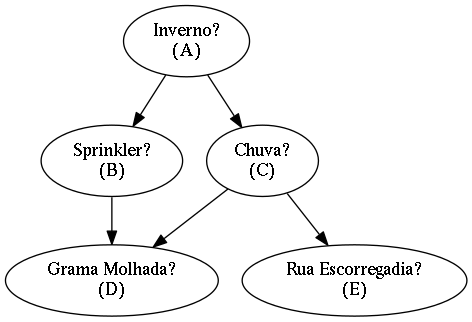
\includegraphics[scale=0.3]{graphs/bn.png}}
  \caption{Uma Rede Bayesiana com cinco variáveis booleanas.}\label{bn-figure}
\end{figure}

\begin{table}[h]
  \begin{center}
    \begin{tabular}{l | l}
      $A$ & $\Theta_A$\\
      \hline
      true & $.6$ \\
      false & $.4$ \\
    \end{tabular}
    \begin{tabular}{l l | l}
      $A$ & $B$ & $\Theta_{B|A}$\\
      \hline
      true & true & $.2$ \\
      true & false & $.8$ \\
      false & true & $.75$ \\
      false & false & $.25$ \\
    \end{tabular}
    \begin{tabular}{l l | l}
      $A$ & $C$ & $\Theta_{C|A}$ \\
      \hline
      true & true & $.8$ \\
      true & false & $.2$ \\
      false & true & $.1$ \\
      false & false & $.9$ \\
    \end{tabular}
    \begin{tabular}{l l l | l}
      $B$ & $C$ & $D$ & $\Theta_{D|B,C}$ \\
      \hline
      true & true & true & $.95$ \\
      true & true & false & $.05$ \\
      true & false & true & $.9$ \\
      true & false & false & $.1$ \\
      false & true & true & $.8$ \\
      false & true & false & $.2$ \\
      false & false & true & $0$ \\
      false & false & false & $1$ \\
    \end{tabular}
    \begin{tabular}{l l | l}
      $C$ & $E$ & $\Theta_{E|C}$ \\
      \hline
      true & true & $.7$ \\
      true & false & $.3$ \\
      false & true & $0$ \\
      false & false & $1$ \\
    \end{tabular}
  \end{center}
  \caption{As CPTs da Rede Bayesiana da Figura~\ref{bn-figure}.}
\end{table}

As tabelas da Rede Bayesiana mostram as probabilidades de cada evento dados os eventos de
dependência. Tais tabelas são chamadas de Tabelas de Probabilidade Condicional (CPTs) por serem
as probabilidades condicionais de cada nó. Denotaremos por $\Theta_{X|Pa(X)}$ a CPT do nó $X$ e
por $\theta_{x\sim X|v\sim Pa(X)}$ um parâmetro, ou seja, uma instanciação de $X$ dada uma
instanciação de $Pa(X)$. Por exemplo, $\theta_{b|\overline{a}}=.8$ indica que a instanciação
$b=true$ e $a=false$ da CPT $\Theta_{B|A}$ é a probabilidade $0.8$.

\begin{example}\label{bn-example}
  Considere que tenhamos a Rede Bayesiana da Figura~\ref{bn-figure} e que desejamos extrair
  conhecimento a partir do nosso modelo. Por exemplo, se soubermos que a rua da casa em que vivemos
  está molhada, teremos mais cuidado ao dirigirmos nela. Ou que se a grama de nosso jardim estiver
  molhada, não a cortaremos nesse dia. Para isso devemos considerar alguns outros eventos que têm
  direta relação com as predições que desejamos inferir. Afinal, se soubermos que hoje choveu,
  temos certeza que a grama ou rua estará molhada. No entanto, mesmo que hoje não tenha chovido,
  é possível que o sistema de sprinklers que instalamos tenha acionado, e portanto a grama estará
  molhada mas a rua não. Além disso, se estivermos no inverno, teremos uma maior chance de chuva
  e provavelmente acionaremos os sprinklers menos vezes devido a isso. Para modelarmos todas estas
  interações, podemos usar uma Rede Bayesiana. Note que há eventos que provavelmente impactariam em
  nosso sistema, porém decidimos não toma-los em conta para simplificarmos o nosso exemplo. Note
  que existe uma aresta entre um par de nó na Rede Bayesiana se e somente se existe uma relação
  direta entre os eventos. Também note que todo ancestral de um nó tem uma relação (mesmo que
  indireta) com o nó em questão.
\end{example}

\subsection{Inferência Exata em Redes Bayesianas}

Acharmos a probabilidade de um certo evento é possível por meio do Teorema da Fatorização, que
apesar de não termos enunciado, tem como resultado a Equação~\ref{factorization-thm}. O Teorema
da Fatorização tem uma relação de se e somente se com a Propriedade Local de Markov (LMP), que
define independências com todas as variáveis não vizinhas dadas as variáveis vizinhas. Podemos
então facilmente derivar~\ref{factorization-thm} por meio da LMP e da Regra da Cadeia de Teoria de
Probabilidade. Vamos relembrar a Equação~\ref{factorization-thm}:

\begin{equation*}
  \Pr(\set{X}) = \prod_{X\in\set{X}} \Pr(X|Pa(X))
\end{equation*}

Aplicando esta equação à Rede Bayesiana da Figura~\ref{bn-figure}, temos

\begin{equation*}
  \Pr(A,B,C,D,E) = \Pr(A)\Pr(B|A)\Pr(C|A)\Pr(D|B,C)\Pr(E|C)
\end{equation*}

A partir da definição de probabilidade condicional, podemos achar qualquer probabilidade de algum
conjunto de eventos $\set{Y}$ dado uma evidência $\set{E}$ dividindo as probabilidades conjuntas

\begin{equation*}
  \Pr(\set{Y}|\set{E}) = \frac{\Pr(\set{Y},\set{E})}{\Pr(\set{E})}
\end{equation*}

Para acharmos as probabilidades conjuntas $\Pr(\set{Y},\set{E})$ e $\Pr(\set{E})$, precisamos
aplicar o Teorema da Fatorização para os eventos relevantes e somar todas as probabilidades que não
temos uma valoração (i.e.\ instanciação) exata. Suponha que $\set{Y}\subseteq\set{X}$ e que
$\set{Y}\cap\set{E}=\emptyset$ e $\set{Y}\cup\set{E}\subset\set{X}$. Temos que

\begin{align*}
  &\Pr(\set{Y},\set{E})=\sum_{v\in\set{X}\setminus(\set{Y}\cup\set{E})} \Pr(v,y,e)\\
  &\Pr(\set{E})=\sum_{v\in\set{X}\setminus\set{E}} \Pr(v,e)\\
\end{align*}

onde $e$ e $y$ são as instanciações de $\set{Y}$ e $\set{E}$ respectivamente. Note que como $v,y,e$
formam uma instanciação completa (em que todas as variáveis estão presentes) podemos aplicar o
Teorema da Fatorização e achar a probabilidade correspondente. É fácil ver que estas operações de
soma e produto são $\bigo(\exp(n))$. De fato, computar a probabilidade exata de uma Rede Bayesiana
no caso geral é NP-difícil. Não só isso como a redução do problema de se computar a probabilidade
exata de uma RB é análoga ao do problema de NP-completude de SAT\@. Se conseguirmos provar que o
problema de se resolver uma sentença booleana é reduzível a um problema com solução eficiente,
teremos uma prova equivalente a de P vs NP~\cite{np-sat}. Por exemplo, computar a seguinte sentença
proposicional tal que o resultado seja verdadeiro para uma instanciação das variáveis da sentença
é, acredita-se, impossível em tempo subexponencial.

\begin{equation*}
  A\vee(B\wedge(C\vee (D\wedge E\vee F)))
\end{equation*}

Portanto, crê-se que o problema de inferência exata em RBs é insolúvel em tempo eficiente.

\begin{example}
  Retomando o Exemplo~\ref{bn-example}, suponha que desejamos saber a probabilidade de a grama
  estar molhada dado que sabemos que hoje choveu e que não estamos no inverno.

  \begin{equation*}
    \Pr(D=true|C=true,A=false)=\frac{\Pr(D=true,C=true,A=false)}{\Pr(C=true,A=false)}
  \end{equation*}

  Usaremos a notação $X=true\equiv X=1$ e $X=false\equiv X=0$. Para cada probabilidade
  conjunta na equação anterior temos

  \begin{align*}
    \Pr(A=0,C=1,D=1)&=\sum_{b,e}\Pr(A=0,b,C=1,D=1,e)=\\
    &=\Pr(A=0,B=0,C=1,D=1,E=0)+\\
    &+\cdots+\\
    &+\Pr(A=0,B=1,C=1,D=1,E=1)\\
  \end{align*}
  \begin{align*}
    \Pr(C=1,A=0)&=\sum_{a,b,d,e}\Pr(A=0,b,C=1,d,e)=\\
    &=\Pr(A=0,B=0,C=1,D=0,E=0)+\\
    &+\cdots+\\
    &+\Pr(A=0,B=1,C=1,D=1,E=1)\\
  \end{align*}

  A probabilidade resultante da divisão das probabilidades conjuntas é o resultado que desejamos
  saber.
\end{example}

\subsection{Inferência aproximada em Redes Bayesianas}

Inferência aproximada pode ser feita de diversos modos. No entanto, por sua própria definição,
o resultado da probabilidade possue um erro que tende a aumentar a cada iteração. Não somente isso,
mas como aprendizado utiliza inferência, o aprendizado torna-se também aproximado.

Existem muitos métodos para inferência aproximada.

\begin{enumerate}
  \item Amostragem estocástica:
    \begin{enumerate}
      \item Lógica,
      \item Por importância de verossimilhança,
      \item Amostragem de Gibbs;
    \end{enumerate}
  \item Propagação de crença;
  \item Algoritmo soma-produto;
  \item entre outros.
\end{enumerate}

Não discutiremos os algoritmos neste relatório.

\section{Sum-Product Networks}

Sabemos que inferência exata em modelos probabilísticos baseados em grafo clássicos é NP-difícil e
portanto intratável no caso geral. Nossa motivação é formularmos um modelo onde inferência exata
seja eficiente. Existem de fato modelos em que computar a probabilidade conjunta ou condicional
exata é sub-exponencial, contudo tais modelos se mostraram muito limitados quanto a sua
generalidade ao representar distribuições.

Inferência e aprendizado em Redes Neurais (RNs) são eficientes, no sentido que são subexponenciais,
quando realizamos o algoritmo de retropropagação em suas estruturas. Seja pelo gradiente da função
ou por EM (expectation-maximization), a complexidade da retropropagação é linear no tamanho do
conjunto de arestas da rede.

Sum-Product Networks (SPNs) são PGMs pois representam uma distribuição de probabilidade. Ao mesmo
tempo, SPNs podem ser vistos como uma RN devido a sua estrutura profunda com camadas ocultas e
operações de soma e produto nos nós. Além disso, inferência é linear no número de arestas da SPN e
portanto aprendizado é tratável. Além disso, se uma SPN obedecer a uma certa propriedade,
inferência por retropropagação será sempre exata e eficiente. Assim como RNs, o aprendizado
profundo de sua estrutura melhora os resultados obtidos, tornando SPNs um modelo atraente para a
área de Inteligência Artificial e principalmente para Incerteza e aprendizado probabilístico.

Antes de discutirmos sobre SPNs, vamos primeiro esclarecer alguns assuntos importantes para o
entendimento de SPNs. Iremos tratar do chamado \textit{network polynomial}, um polinômio em função
das variáveis de uma distribuição de probabilidade que representa a função que desejamos
representar pela SPN\@. Em seguida trataremos da descrição da estrutura de uma SPN e em seguida
daremos uma rápida explicação de como se computar inferência exata em sua estrutura pelo algoritmo
de retropropagação. Finalmente, discutiremos brevemente sobre aprendizagem.

\subsection{Network polynomial}

Sabemos que uma Rede Bayesiana pode ser representada por CPTs, e que cada CPT é uma variável da
rede. Considere a rede da Figura~\ref{simple-bn} como exemplo.

\begin{figure}[h]
  \centering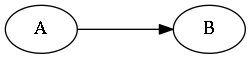
\includegraphics[scale=0.3]{graphs/simple_bn.png}
  \caption{Uma simples Rede Bayesiana $A\to B$.}\label{simple-bn}
\end{figure}

\begin{table}[h]
  \begin{center}
    \begin{tabular}{l | l}
      $A$ & $\Theta_A$ \\
      \hline
      true & $.7$ \\
      false & $.3$ \\
    \end{tabular}
    \begin{tabular}{l l | l}
      $A$ & $B$ & $\Theta_{B|A}$ \\
      \hline
      true & true & $.2$ \\
      true & false & $.8$ \\
      false & true & $.6$ \\
      false & false & $.4$ \\
    \end{tabular}
  \end{center}
\end{table}

\begin{definition}
  O polinômio da rede (\emph{network polynomial}) é a função da soma de todas as instanciações da
  distribuição conjunta de uma Rede Bayesiana multiplicadas com as variáveis indicadoras de cada
  variável.

  \begin{equation*}
    f(\set{X})=\sum_{\set{x}\sim\set{X}} \lambda_{\set{x}}\theta_{\set{x}|v\sim Pa(\set{x})}
  \end{equation*}

  Uma variável indicadora é $1$ se a variável é consistente com a instanciação e 0 caso contrário.
  Caso a variável não seja instanciada, a variável indicadora é $1$.
\end{definition}

\begin{example}
  Denotaremos $a$ se $A=true$ e $\overline{a}$ se $A=false$. O polinômio da rede da
  Figura~\ref{simple-bn} é:

  \begin{equation*}
    f(A,B)=\lambda_a\lambda_b\theta_a\theta_{b|a}+\lambda_{\overline{a}}\lambda_b
    \theta_{\overline{a}}\theta_{b|\overline{a}}+\lambda_a\lambda_{\overline{b}}\theta_a
    \theta_{\overline{b}|a}+\lambda_{\overline{a}}\lambda_{\overline{b}}
    \theta_{\overline{a}}\theta_{\overline{b}|\overline{a}}
  \end{equation*}

  Se tivermos $a$ e $\overline{b}$, as variáveis indicadoras são $\lambda_a=\lambda_{\overline{b}}=
  1$ e $\lambda_b=\lambda_{\overline{a}}=0$ e a probabilidade $\Pr(a,\overline{b})$ é

  \begin{align*}
    \Pr(a,\overline{b})=f(a,\overline{b})=\theta_a\theta_{\overline{b}|a}
  \end{align*}

  Se desejassemos a probabilidade $\Pr(b)$, as variáveis indicadoras teriam valores $\lambda_a=
  \lambda_{\overline{a}}=\lambda_b=1$ e $\lambda_{\overline{b}}=0$.
\end{example}

\subsection{Estrutura de uma Sum-Product Network}

\begin{definition}
  Uma SPN $S$ é um DAG com três tipos de nós: soma, produto e indicadores. Todo nó indicador é uma
  folha. Todo nó soma tem pais produto, e todo nó produto tem pais soma. Toda aresta com destino a
  um nó soma tem uma aresta com um peso associado. O valor de um nó soma $i$ é $\sum_{j\in Ch(i)}
  w_{ij}v_j$ e o valor de um nó produto $i$ é $\prod_{j\in Ch(i)}v_j$, onde $Ch(i)$ é o conjunto
  de filhos de $i$, $v_i$ é o valor do nó $i$ e $w_{ij}$ é o peso associado a aresta $i\to j$. Uma
  SPN representa um \emph{network polynomial} de uma distribuição de probabilidade, e os
  indicadores da função são as folhas da SPN\@. O valor de uma SPN é o valor do nó raíz.
\end{definition}

\begin{figure}[h]
  \centering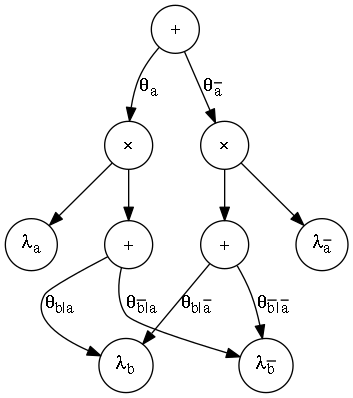
\includegraphics[scale=0.4]{graphs/simple_spn.png}
  \caption{Estrutura da SPN que representa a \textit{network polynomial} da
  Figura~\ref{simple-bn}.}\label{simple-spn}
\end{figure}

Ao contrário dos CPGMs que possuem uma estrutura que explicitamente representa a distribuição de
probabilidade, SPNs tem sua representatividade implícita por uma função polinomial, assim como
Redes Neurais.

\subsection{Inferência por Retropropagação}

Devido a sua estrutura semelhante a de Redes Neurais, podemos computar inferência exata por meio
do método de retropropagação, assim como em RNs.

Para computarmos a probabilidade marginal $\Pr(\set{Y})$, utilizamos as variáveis indicadoras de
forma consistente com a instanciação $\set{Y}$. Por exemplo, seja $\set{Y}=\{X_1=true\}$ e sejam
as variáveis da rede $\set{X}=\{X_1,X_2\}$. Então queremos a probabilidade $\Pr(X_1=true)$.
Portanto, as variáveis indicadores serão $\lambda_{X_1}=1$, $\lambda_{\overline{X}_1}=0$,
$\lambda_{X_2}=\lambda_{\overline{X}_2}=1$.

\begin{figure}[h]
  \centering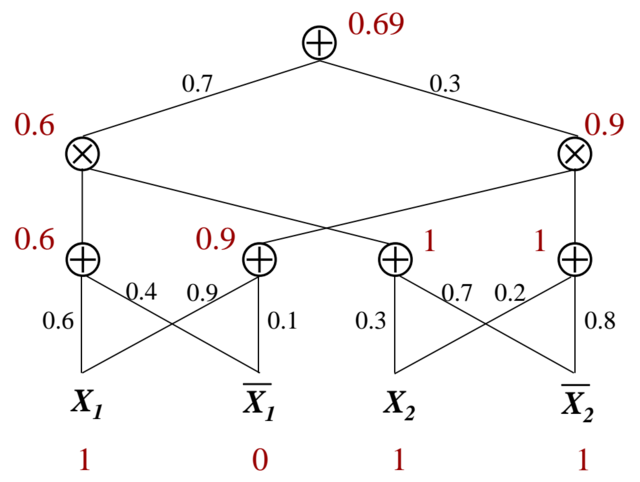
\includegraphics[scale=0.3]{imgs/marginals.png}
  \caption{O valor da SPN é o valor do nó raíz. Neste caso, o valor da SPN $S=\Pr(X_1=true)=0.69$.}
\end{figure}

Para acharmos a probabilidade correspondente, fixamos os valores das folhas (variáveis indicadoras)
para seus valores consistentes com a nossa instanciação e em seguida computamos o valor da raíz
recursivamente. Probabilidades posteriores podem então serem computadas pela definição de
probabildade condicional após achadas as probabilidades marginais.

\subsection{Aprendizado}

Aprendizado em SPNs é dividido em duas classes: paramétrico~\cite{poon-domingos} e
estrutural~\cite{gens-domingos}.

Na primeira classe, temos uma estrutura fixa com uma quantidade de camadas ocultas razoavelmente
grande e desejamos aprender os pesos das arestas da SPN\@. Assim como em Redes Neurais, é possível
utilizarmos o gradiente para encontrarmos um máximo local. Outro possível método é utilizarmos EM
(expectation-maximization).

Na segunda classe, desejamos criar uma estrutura com um grande número de camadas ocultas. Podemos
arranjar as camadas por meio da identificação de independências entre as variáveis.

\section{Planejamento}

Planeja-se estudar os seguintes tópicos:

\begin{enumerate}
  \item \textit{Background} teórico (PGMs clássicos, probabilidade)
  \item Inferência em SPNs
    \begin{enumerate}
      \item Função de partição
      \item Marginais
      \item MAP
      \item MPE
    \end{enumerate}
  \item Aprendizagem em SPNs
    \begin{enumerate}
      \item Paramétrica
      \item Estrutural
    \end{enumerate}
\end{enumerate}

Por ser um tópico bem recente e avançado, a maior parte do estudo será teórico.

%--------------------------------------------------------------------------------------------------

\newpage
\appendix

\newpage

\printbibliography[]

\end{document}
